\documentclass[12pt]{article}
\usepackage[utf8]{inputenc}
\usepackage[greek,english]{babel}
\usepackage{alphabeta}
\usepackage{fancyhdr}
\usepackage{listings}
\usepackage{mathtools}
\usepackage{xcolor}
\usepackage{float}
\usepackage{siunitx}
\usepackage[margin=0.5in]{geometry}
\usepackage[backend=bibtex]{biblatex}

\lstset {
        basicstyle=\ttfamily,
        columns=fullflexible,
        breaklines=true,
        keepspaces=true,
	showstringspaces=false
}

\title{Εργαστήριο Ηλεκτρονικού Εμπορίου και Επιχειρηματικότητας -- Εργασία 1}
\author{Χρήστος Μαργιώλης -- 19390133}
\date{Μάιος 2024}

\begin{document}

\begin{titlepage}
        \maketitle
        \begin{figure}[t!]
        \begin{center}
        
\includegraphics[scale=0.3]{./res/uniwalogo.png} \\
        \Large
        \textbf{Πανεπιστήμιο Δυτικής Αττικής} \\
        \large
        Τμήμα Μηχανικών Πληροφορικής και Ηλεκτρονικών Υπολογιστών
        \end{center}
        \end{figure}
\end{titlepage}

\renewcommand{\contentsname}{Περιεχόμενα}
\tableofcontents
\pagebreak

%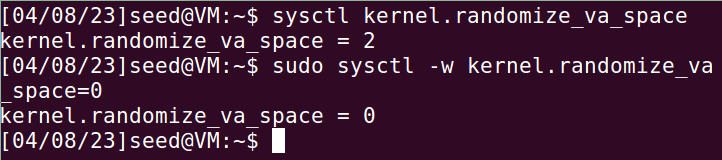
\includegraphics[width=\textwidth]{res/aslr.png} \\

\section{Περίληψη εργασίας}

ΠΡΟΣΟΧΗ: Η εργασία έγινε σε FreeBSD αντί για Windows, διότι βρίσκομαι εκτός Ελλάδας κατά την συγγραφή την
εργασίας και δεν έχω πρόσβαση σε Windows υπολογιστή.

Η παρούσα εργασία έχει ως στόχο την εξοικείωση στην εγκατάσταση, διασύνδεση και
χρήση διαφόρων βασικών τεχνολογιών που χρησιμοποιούνται στον τομέα του
προγραμματισμού διαδικτυακών εφαρμογών.

\section{Α1: Εγκατάσταση Apache HTTP server}

Εγκατάσταση Apache 2.4:

\begin{lstlisting}
# pkg install apache24
\end{lstlisting}

Δημιουργία root directory για την ιστοσελίδα μας και ανάθεση του χρήστη
\lstinline{www} (Apache server) ως κατόχου του directory:

\begin{lstlisting}
# mkdir ecom1
# chown -R www ecom1/
\end{lstlisting}

Τροποποίηση των απαραίτητων \lstinline{DocumentRoot} στο αρχείο
\lstinline{http.conf}, ώστε ο server να βρει το directory της ιστοσελίδας και
να κάνει χρήση της σωστής IP:

\begin{lstlisting}
# nvim /usr/local/etc/apache24/httpd.conf
...
ServerName localhost:80
...
DocumentRoot "/usr/home/christos/ecom1"
<Directory "/usr/home/christos/ecom1">
\end{lstlisting}

Επιβεβαίωση της ορθότητας του config αρχείου:

\begin{lstlisting}
# httpd -t
Syntax OK
\end{lstlisting}

Εκκίνηση του server:

\begin{lstlisting}
# service apache24 onestart
Performing sanity check on apache24 configuration:
Syntax OK
Starting apache24.
\end{lstlisting}

Επιβεβαίωση ότι ο server ακούει στο port 80:

\begin{lstlisting}
# sockstat -4 -l -P tcp -p 80
USER     COMMAND    PID   FD  PROTO  LOCAL ADDRESS         FOREIGN ADDRESS
www      httpd      23853 4   tcp4   *:80                  *:*
www      httpd      23852 4   tcp4   *:80                  *:*
www      httpd      23851 4   tcp4   *:80                  *:*
www      httpd      23850 4   tcp4   *:80                  *:*
www      httpd      23849 4   tcp4   *:80                  *:*
root     httpd      23848 4   tcp4   *:80                  *:*
\end{lstlisting}

\section{Α2: Εγκατάσταση PHP και διασύνδεση με το Apache}

Εγκατάσταση της PHP 8.2 και του Apache module:

\begin{lstlisting}
# pkg install php82 mod_php82
\end{lstlisting}

Δημιουργία \lstinline{php.ini} αρχείο, βασισμένο στo
\lstinline{php.ini-development}:

\begin{lstlisting}
# cp /usr/local/etc/php.ini-development /usr/local/etc/php.ini
\end{lstlisting}

Επιβεβαίωση ότι το πρόγραμμα κελύφους \lstinline{php} τρέχει χωρίς προβλήματα:

\begin{lstlisting}
# php -v
PHP 8.2.19 (cli) (built: May 21 2024 02:10:26) (NTS)
Copyright (c) The PHP Group
Zend Engine v4.2.19, Copyright (c) Zend Technologies
\end{lstlisting}

Τροποποίση \lstinline{httpd.conf} ώστε να γίνει η διασύνδεση του Apache με την
PHP:

\begin{lstlisting}
# nvim /usr/local/etc/apache24/httpd.conf
...
<IfModule dir_module>
    DirectoryIndex index.html index.php
<FilesMatch "\.php$">
    SetHandler application/x-httpd-php
</FilesMatch>
<FilesMatch "\.phps$">
    SetHandler application/x-httpd-php-source
</FilesMatch>
</IfModule>
\end{lstlisting}

Δημιουργία αρχείο δοκιμής στην ιστοσελίδα, ώστε να επιβεβαιώσουμε την
διασύνδεση Apache - PHP:

\begin{lstlisting}
# echo "<?php phpinfo(); ?>" > ecom1/info.php
\end{lstlisting}

Επανεκκίνηση του Apache:

\begin{lstlisting}
# httpd -t
# service apache24 onerestart
\end{lstlisting}

Σε ένα παράθυρο browser, πηγαίνουμε στην διεύθυνση
\lstinline{localhost:80/info.php} για να δούμε αν το αρχείο δοκιμής λειτουργεί
όπως περιμένουμε:

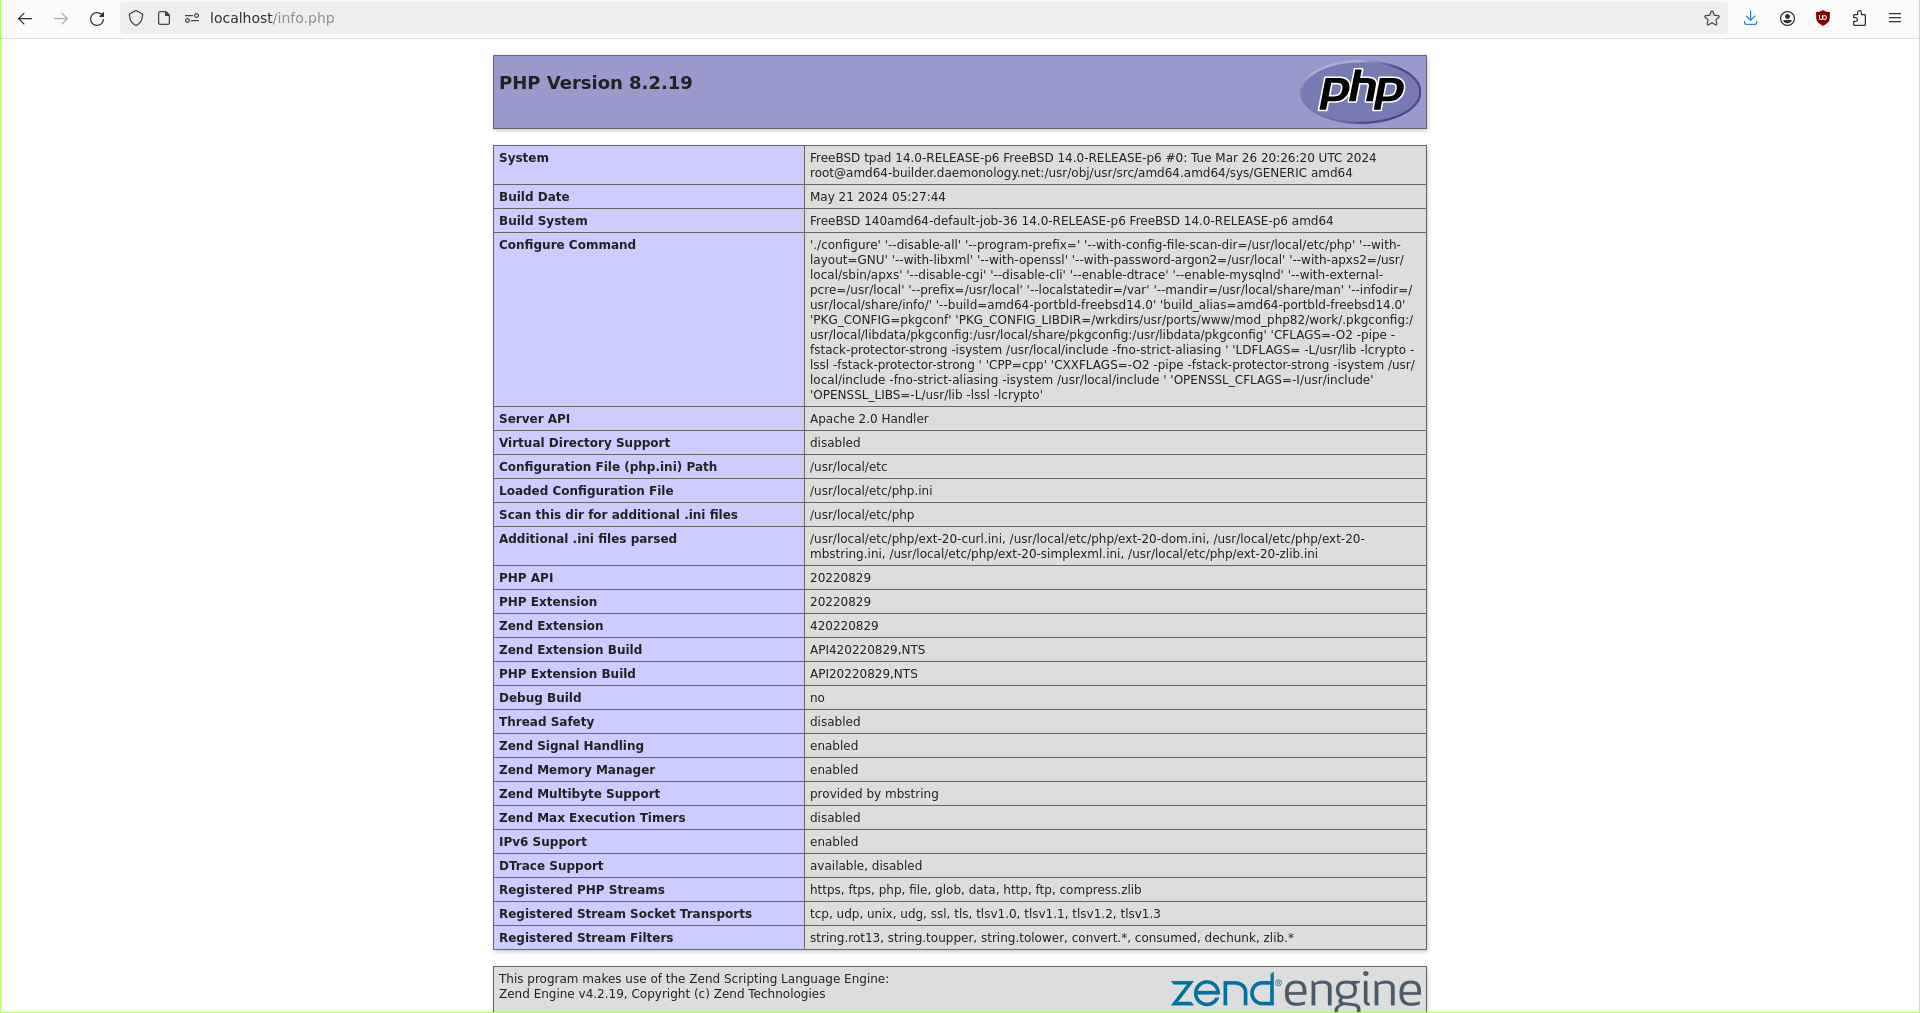
\includegraphics[width=\textwidth]{res/phpinfo.png} \\

\section{Α3: Εγκατάσταση SQLite και διασύνδεση με την PHP}

Εγκατάσταση SQLite3 και του PHP module:

\begin{lstlisting}
# pkg install sqlite3 php82-sqlite3
\end{lstlisting}

Επιβεβαίωση λειτουργίας:

\begin{lstlisting}
# sqlite3 --version
3.45.1 2024-01-30 16:01:20 e876e51a0ed5c5b3126f52e532044363a014bc594cfefa87ffb5b82257ccalt1 (64-bit)
\end{lstlisting}

Δημιουργία βάσης δεδομένων από την γραμμή εντολών:

\begin{lstlisting}
# sqlite3 ecom1/foo.db
SQLite version 3.45.1 2024-01-30 16:01:20
Enter ".help" for usage hints.
sqlite> .databases
main: /usr/home/christos/ecom1/foo.db r/w
sqlite> create table users (id integer, name text);
sqlite>
\end{lstlisting}

Υλοποίηση προγράμματος PHP το οποίο δημιουργεί μια βάση δεδομένων και τυπώνει
τα περιεχόμενά της:

\begin{lstlisting}
# cat > ecom1/sqlite.php
<?php

$db = new SQLite3("foo.db");
$db->exec("INSERT INTO users (id, name) VALUES (1, 'christos')");
$db->exec("INSERT INTO users (id, name) VALUES (2, 'john')");
$db->exec("INSERT INTO users (id, name) VALUES (3, 'mark')");
$res = $db->query("SELECT * FROM users");
while (($row = $res->fetchArray(SQLITE3_ASSOC)) != false)
	print_r($row);
$db->exec("DELETE FROM users");

?>
^D
\end{lstlisting}

Επανεκκίνηση του Apache:

\begin{lstlisting}
# service apache24 onerestart
\end{lstlisting}

Εκτέλεση προγράμματος \lstinline{sqlite.php} στον browser:

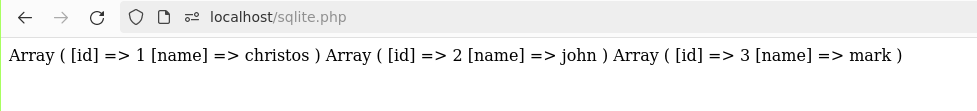
\includegraphics[width=\textwidth]{res/sqlite.png} \\

\section{Α4: Εγκατάσταση MySQL/MariaDB και διασύνδεση με την PHP}

Εγκατάσταση της MySQL 8.4 και του κατάλληλου PHP module:

\begin{lstlisting}
# pkg install mysql84-server php82-mysqli
\end{lstlisting}

Εκκίνηση της MySQL:

\begin{lstlisting}
# service mysql-server onestart
# mysql_secure_installation
\end{lstlisting}

Επιβεβαίωση λειτουργίας της MySQL:

\begin{lstlisting}
# mysql --version
mysql  Ver 8.4.0 for FreeBSD14.0 on amd64 (Source distribution)
\end{lstlisting}

Επανεκκίνηση του Apache:

\begin{lstlisting}
# service apache24 onerestart
\end{lstlisting}

Υλοποίηση προγράμματος PHP το οποίο δημιουργεί μια βάση δεδομένων και τυπώνει
τα περιεχόμενά της:

\begin{lstlisting}
# cat > ecom1/mysql.php
<?php
$conn = new mysqli("localhost", "root", "foobar123#", "foo");
if ($conn->connect_error)
	die("Connection failed: " . $conn->connect_error);

$conn->query("CREATE TABLE users (id INTEGER, name TEXT)");
$conn->query("INSERT INTO users (id, name) VALUES (1, 'christos')");
$conn->query("INSERT INTO users (id, name) VALUES (2, 'john')");
$conn->query("INSERT INTO users (id, name) VALUES (3, 'mark')");

$res = mysqli_query($conn, "SELECT * FROM users");
while ($row = mysqli_fetch_assoc($res))
	print_r($row);

$conn->close();
?>
^D
\end{lstlisting}

Εκτέλεση προγράμματος \lstinline{mysql.php} στον browser:

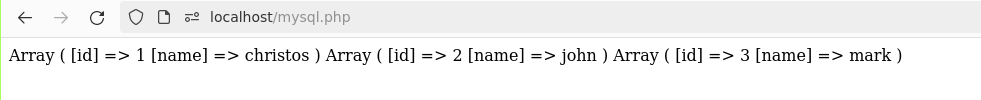
\includegraphics[width=\textwidth]{res/mysql.png} \\

\section{Α5: Εγκατάσταση Perl και διασύνδεση με Apache και SQLite η MySQL}

Εγκάτασταση του Apache Pearl module:

\begin{lstlisting}
# pkg install ap24-mod_perl2
\end{lstlisting}

\section{Προσάρτημα}

Το μόνο αρχείο που χρειάστηκε τροποποίηση είναι το \lstinline{httpd.conf}, του
οποίου οι αλλαγές φαίνονται στις παραπάνω ενότητες. Τα υπόλοιπα αρχεία
δημιουργήθηκαν/τροποποιήθηκαν αυτόματα κατά την εγκατάσταση των προγραμμάτων.

\end{document}
